\section{Methodology}
\label{sec:methodology}

\subsection{Model Architecture}
\label{sec:architecture}

We employ two deep 3D ResNet variants, differing in initial channel width and depth. Both use a stem of Conv3D + BatchNorm + ReLU + MaxPool3D(2), followed by three stages each containing a Residual Block and a Downsampling Block, a final Conv3D + BN + ReLU, AdaptiveAvgPool3D(2$\times$2$\times$2), and a classification head.

\noindent\textbf{Residual Block:}
\begin{equation}
    \mathcal{R}(x) = \text{ReLU}\big(x + \text{BN}(\text{Conv}(\text{ReLU}(\text{BN}(\text{Conv}(x)))))\big)
\end{equation}
where both convolutions are 3$\times$3$\times$3 with padding=1, preserving spatial dimensions.

\noindent\textbf{Downsampling Block:}
\begin{equation}
    \mathcal{D}(x) = \mathcal{R}\big(\text{BN}(\text{Conv}_{3\times3\times3,\text{stride}=2}(x))\big)
\end{equation}
which halves spatial resolution while doubling channels.

\noindent\textbf{Net3dR-v25 (Regular):} Initial 16 channels.
\begin{align*}
    \text{Stem:} & \quad 1 \xrightarrow{\text{Conv+MP}} 16 \text{ channels, } 40^3 \\
    \text{Stage 1:} & \quad \mathcal{R}(16) \to \mathcal{D}(16\!\to\!32) \to 32 \text{ ch, } 20^3 \\
    \text{Stage 2:} & \quad \mathcal{D}(32\!\to\!64) \to 64 \text{ ch, } 10^3 \\
    \text{Stage 3:} & \quad \text{Conv}(64\!\to\!128) \to 128 \text{ ch, } 10^3 \\
    \text{Head:} & \quad \text{AvgPool}(2^3) \to \text{FC}(1024\!\to\!256) \to \text{FC}(256\!\to\!1)
\end{align*}
Total parameters: \textbf{845,089}.

\noindent\textbf{Net3dBig-v25 (Wide):} Initial 20 channels.
\begin{align*}
    \text{Stem:} & \quad 1 \xrightarrow{\text{Conv+MP}} 20 \text{ channels, } 40^3 \\
    \text{Stage 1:} & \quad \mathcal{R}(20) \to \mathcal{D}(20\!\to\!40) \to 40 \text{ ch, } 20^3 \\
    \text{Stage 2:} & \quad \mathcal{D}(40\!\to\!80) \to 80 \text{ ch, } 10^3 \\
    \text{Stage 3:} & \quad \text{Conv}(80\!\to\!160) \to 160 \text{ ch, } 10^3 \\
    \text{Head:} & \quad \text{AvgPool}(2^3) \to \text{FC}(1280\!\to\!320) \to \text{FC}(320\!\to\!1)
\end{align*}
Total parameters: \textbf{1,319,721}.

\begin{figure}[H]
    \centering
    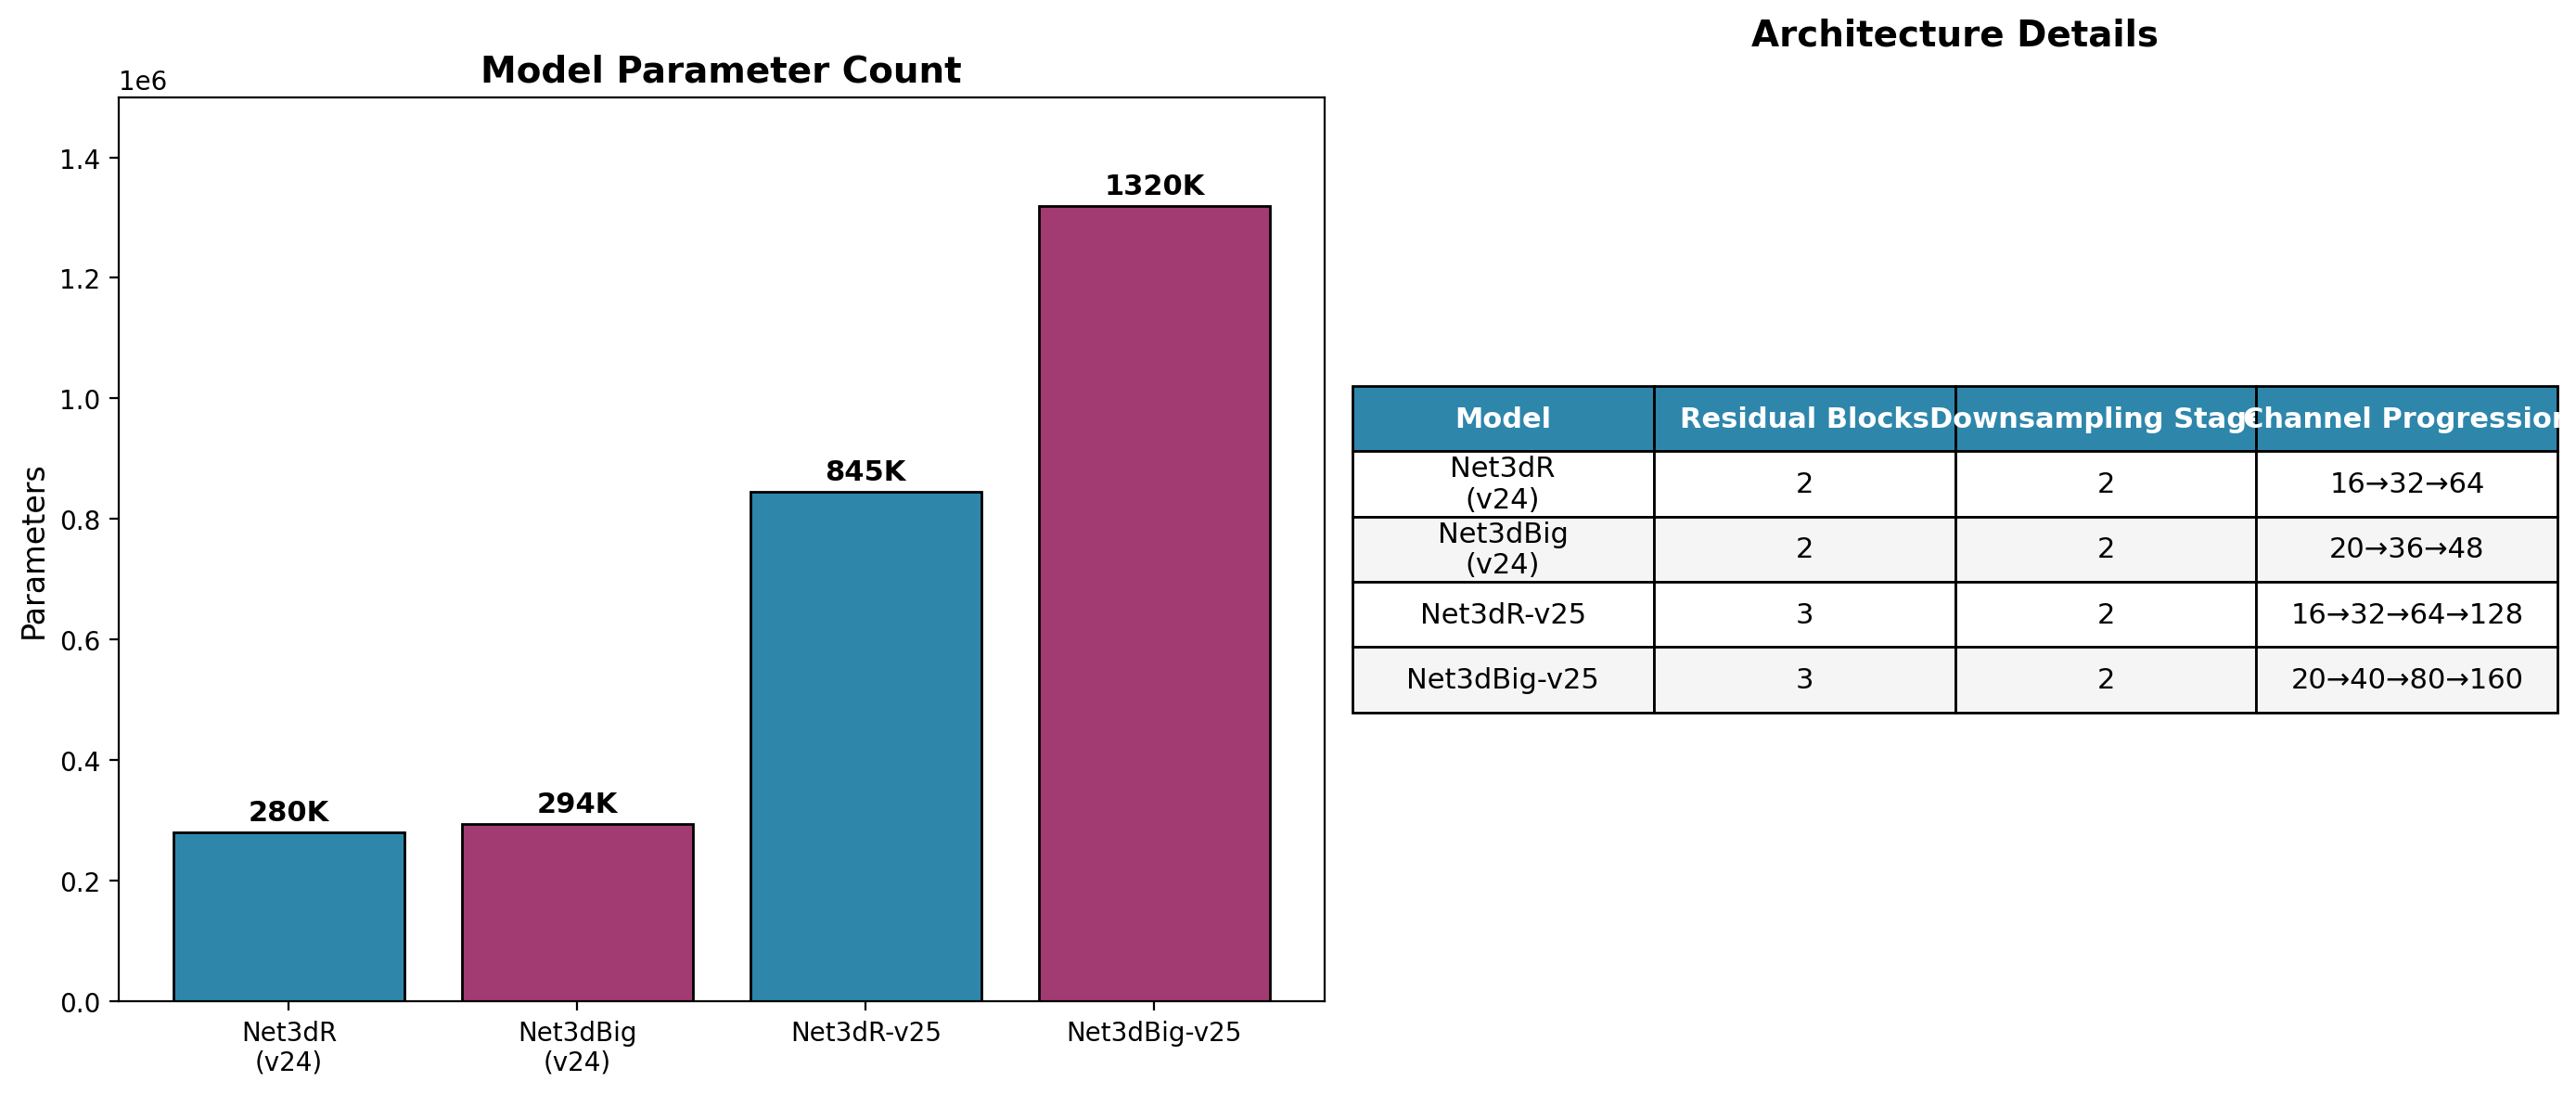
\includegraphics[width=0.95\linewidth]{figures/architecture_comparison.png}
    \caption{Architecture comparison across versions. (Left) Parameter count: v24 models (280K/294K) vs. v25 models (845K/1.3M). (Right) Architecture details table showing block counts, downsampling stages, and channel progressions.}
    \label{fig:architecture}
\end{figure}

Table~\ref{tab:architecture} summarizes the evolution across versions.

\begin{table}[H]
\centering
\caption{Model architecture evolution from v23 to v25.}
\label{tab:architecture}
\begin{tabular}{lccc}
\toprule
\textbf{Component} & \textbf{v23} & \textbf{v24} & \textbf{v25} \\
\midrule
Architecture family & Net3dR / Net3dBig & Net3dR / Net3dBig & \textbf{Deep ResNet v25} \\
Residual blocks & 2 & 2 & \textbf{3} \\
Downsampling stages & 2 & 2 & \textbf{3} \\
Max channels & 64 / 48 & 64 / 48 & \textbf{128 / 160} \\
Parameters per model & 280K / 294K & 280K / 294K & \textbf{845K / 1.3M} \\
Models in ensemble & 6 (3+3) & 6 (3+3) & \textbf{10 (5+5)} \\
Seeds per architecture & 3 & 3 & \textbf{5} \\
Input resolution & 32$\times$40$\times$48 & 80$^3$ & 80$^3$ \\
Crop/Full volume & Crop & Full & Full \\
\bottomrule
\end{tabular}
\end{table}

\subsection{Training Configuration}
\label{sec:training}

\noindent\textbf{Loss Function.} Label-smoothing binary cross-entropy with mixup:
\begin{equation}
    \mathcal{L} = \mathbb{E}_{(\mathbf{x},y)\sim\mathcal{D}} \Big[ \ell_{\text{BCE}}\big(f(\text{Mix}_\alpha(\mathbf{x})), \text{Mix}_\alpha(y)\big) \Big]
\end{equation}
where $\text{Mix}_\alpha(\mathbf{x}) = \lambda \mathbf{x}_i + (1-\lambda)\mathbf{x}_j$, $\lambda \sim \text{Beta}(\alpha,\alpha)$, $\alpha=0.2$. Label smoothing: $y_{\text{smooth}} = y(1-\epsilon) + 0.5\epsilon$, $\epsilon=0.05$.

\noindent\textbf{Optimization.}
\begin{itemize}
    \item Optimizer: AdamW ($\text{lr}=10^{-4}$, $\text{weight\_decay}=10^{-4}$)
    \item Scheduler: CosineAnnealingLR ($T_{\text{max}}=100$ epochs)
    \item Batch size: 8 (gradient accumulation $\times$3 $\to$ effective batch 24)
    \item Mixed precision: AMP (FP16)
    \item Gradient clipping: max\_norm=1.0
    \item Early stopping: patience=20 epochs on validation loss
    \item Max epochs: 100
\end{itemize}

\noindent\textbf{Data Augmentation (Training Only).}
\begin{itemize}
    \item Random flips: 50\% probability on each axis (X, Y, Z)
    \item Random scale: Uniform(0.93, 1.07)
    \item Random shift: Uniform(-0.02, 0.02) per voxel
    \item Mixup: $\alpha=0.2$ (applied per-batch)
    \item Label smoothing: $\epsilon=0.05$
\end{itemize}

\noindent\textbf{Ensemble Strategy.}
\begin{itemize}
    \item 5 random seeds per architecture: \{42, 777, 2024, 1984, 100\} for Net3dR; \{2025, 314, 271, 1337, 999\} for Net3dBig
    \item Each seed trained independently on all 5 folds (50 models total)
    \item Fold weights averaged for final inference models
\end{itemize}

\subsection{Cross-Validation Strategy}
\label{sec:cv}
We employ \textbf{StratifiedGroupKFold} with 5 folds:
\begin{itemize}
    \item Groups: 15 scanner sites (prevents site-level leakage)
    \item Stratification: Binary label (pathological/normal)
    \item Shuffle: True, random\_state=42
    \item Fold sizes: 272--273 validation / 1,089--1,090 training
\end{itemize}

This ensures no scanner appears in both training and validation within any fold, providing an unbiased estimate of generalization to unseen sites.

\subsection{Inference Pipeline}
\label{sec:inference}

\begin{enumerate}
    \item \textbf{Load \& Preprocess:} Identical to training preprocessing (RAS, resample to 2.0~mm, COM-center on 80$^3$).
    \item \textbf{Coarse Rotation Alignment:} Search $\pm$5$^\circ$ in 2$^\circ$ steps on 3 planes (sagittal YZ, coronal XZ, axial XY) via NCC against atlas template. Best rotation applied.
    \item \textbf{Translation Alignment:} Search $\pm$4 voxels in 3D via NCC against shifted template. Best shift applied.
    \item \textbf{Percentile Normalization:} Clip to [1st, 99th] percentile, min-max scale to [0, 1].
    \item \textbf{Test-Time Augmentation (15 views):}
    \begin{itemize}
        \item 1 base view
        \item 6 translation views: roll $\pm$1 voxel on X, Y, Z axes
        \item 8 rotation views: $\pm$2$^\circ$, $\pm$4$^\circ$ on sagittal (YZ) and coronal (XZ) planes
    \end{itemize}
    \item \textbf{Ensemble:} Average sigmoid probabilities across 10 models $\times$ 15 views = 150 predictions.
    \item \textbf{Platt Calibration:} $p_{\text{cal}} = \sigma(a \cdot \text{logit}(p) + b)$ with $a=1.45, b=0.20$ fit on OOF ensemble.
\end{enumerate}

\begin{figure}[H]
    \centering
    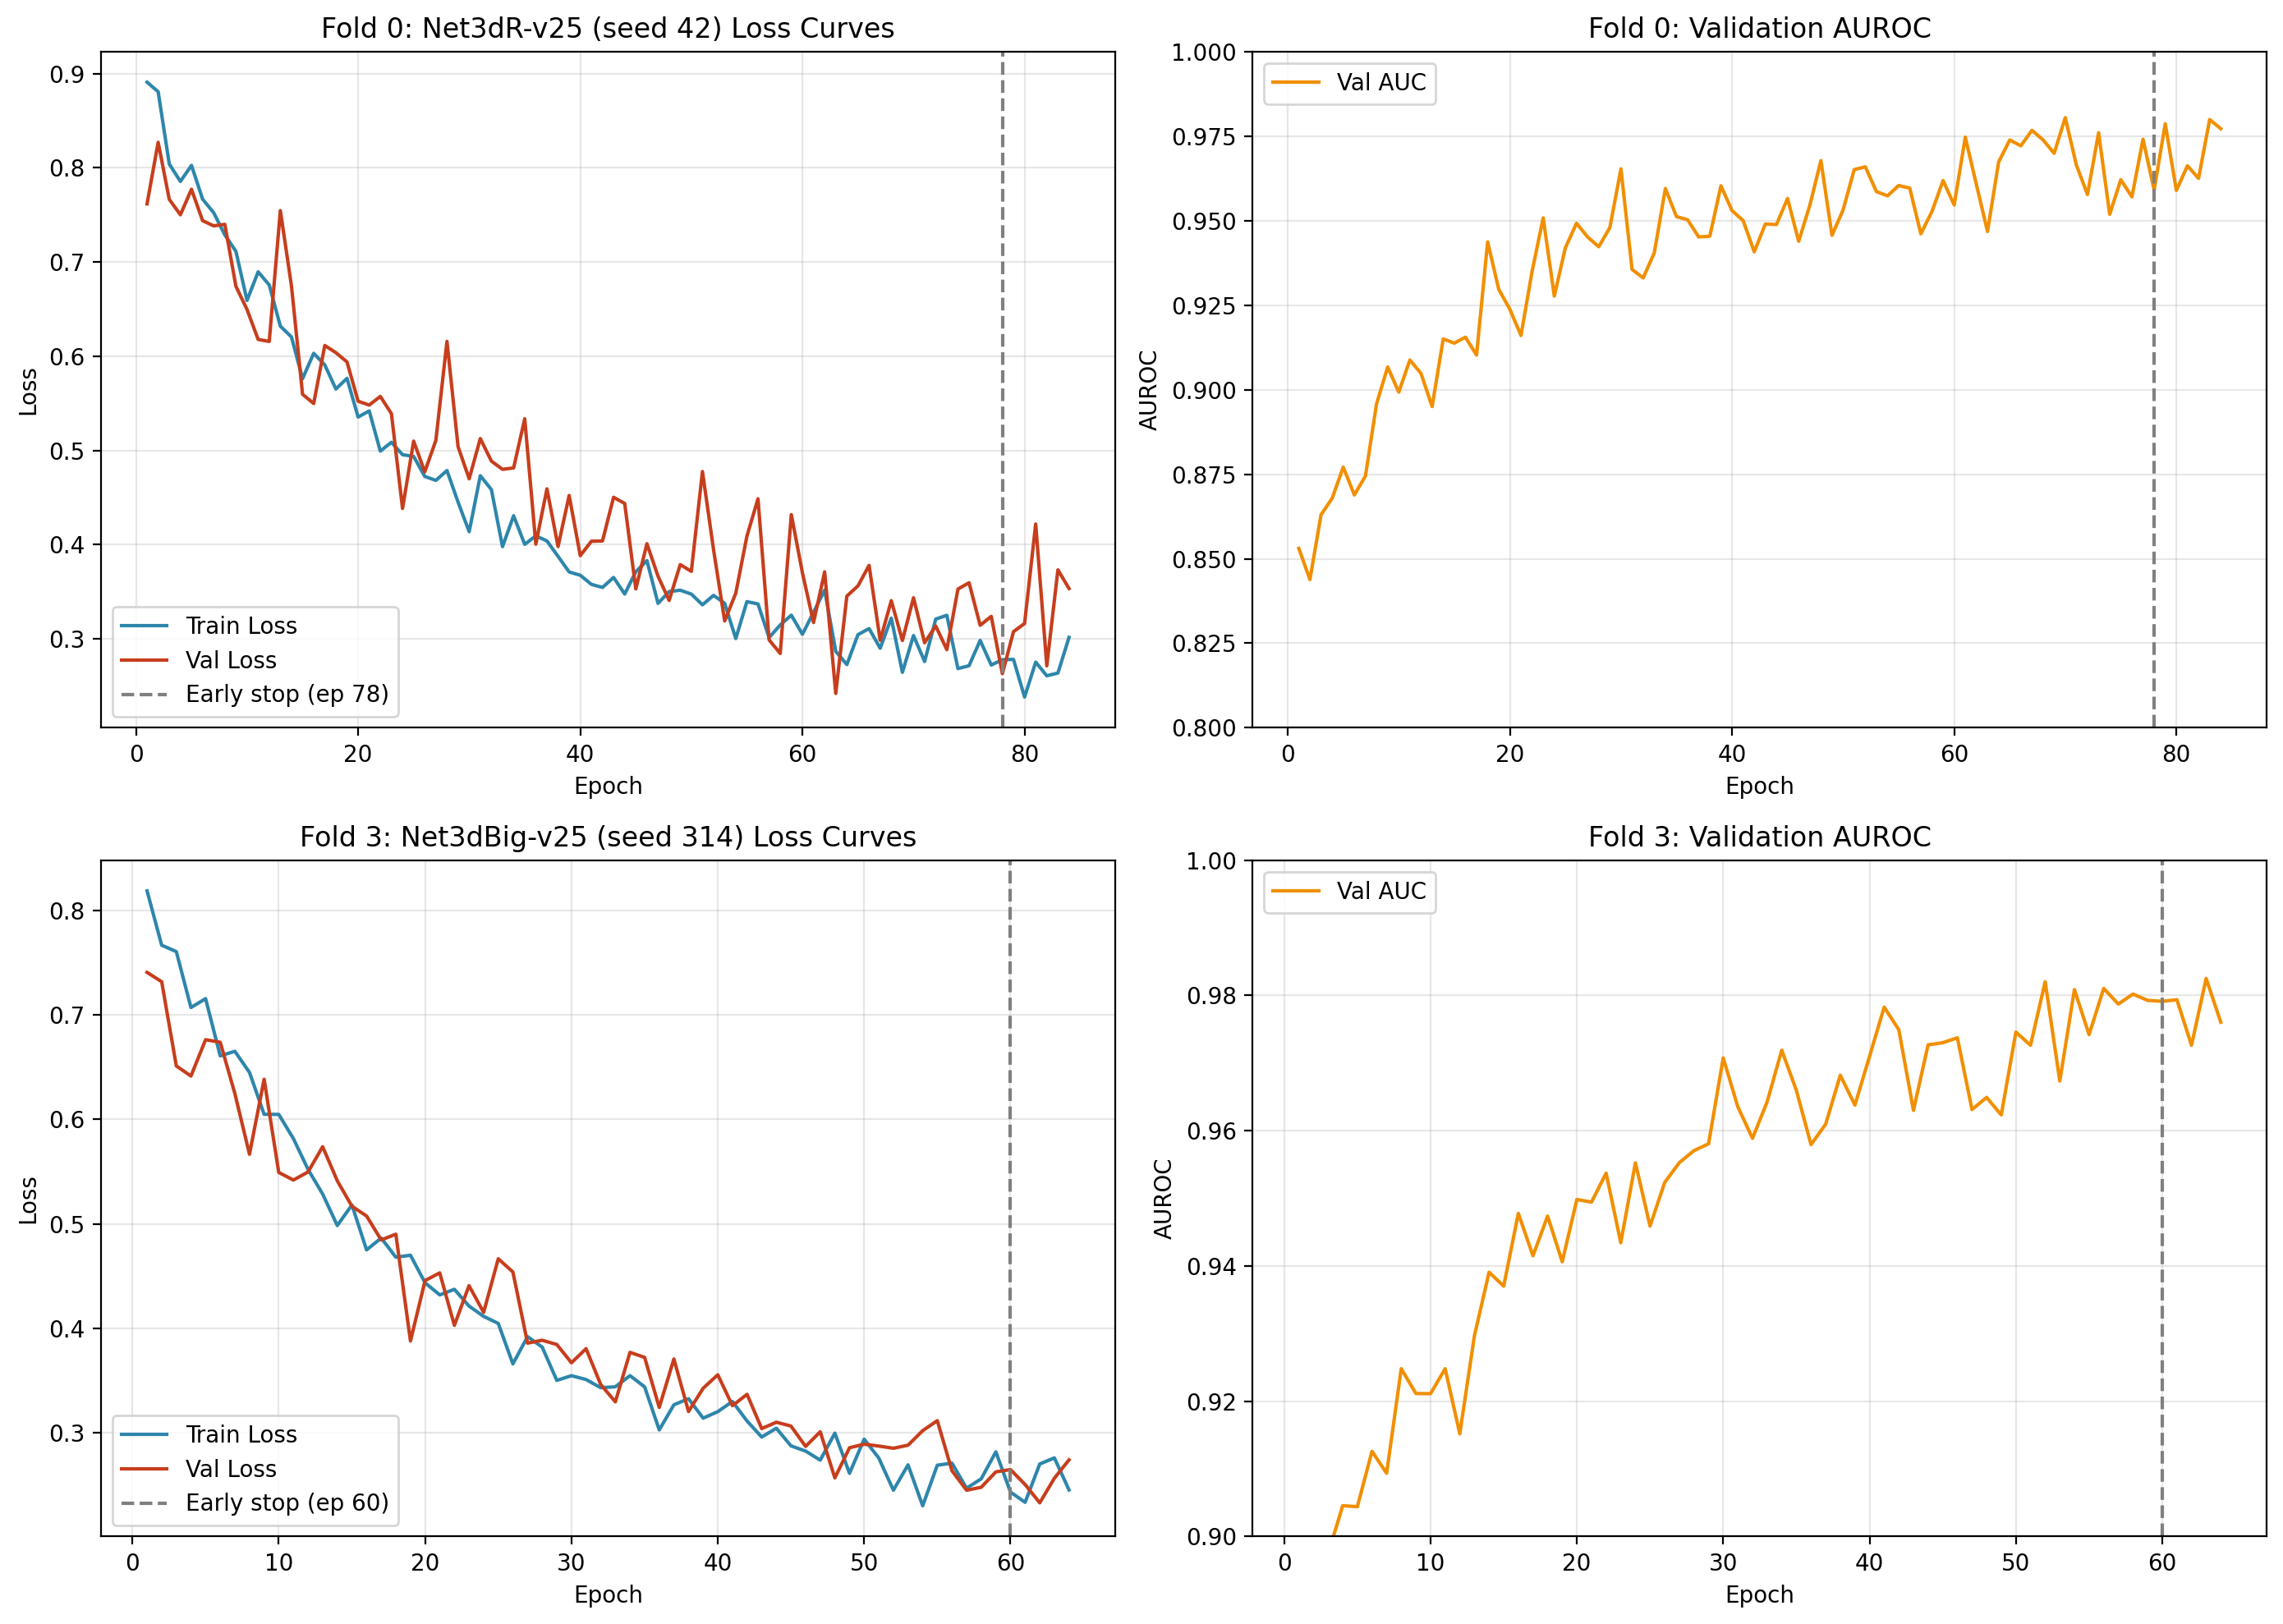
\includegraphics[width=0.9\linewidth]{figures/training_curves.png}
    \caption{Training curves for two representative models. (Top) Net3dR-v25 Fold 0 seed 42: early stop at epoch 78, val AUC reaches 0.96. (Bottom) Net3dBig-v25 Fold 3 seed 314: early stop at epoch 60, val AUC reaches 0.97. Shaded regions show typical variance across seeds.}
    \label{fig:training_curves}
\end{figure}

\subsection{Calibration}
\label{sec:calibration}
Post-hoc Platt scaling is fit on the OOF ensemble predictions (1,362 samples) by grid search over $a \in [0.5, 2.0]$, $b \in [-1.0, 1.0]$ minimizing LogLoss. Optimal parameters: $a=1.45, b=0.20$. This improves LogLoss from 0.2618 to \textbf{0.2453} while AUROC remains 0.9610.

\begin{figure}[H]
    \centering
    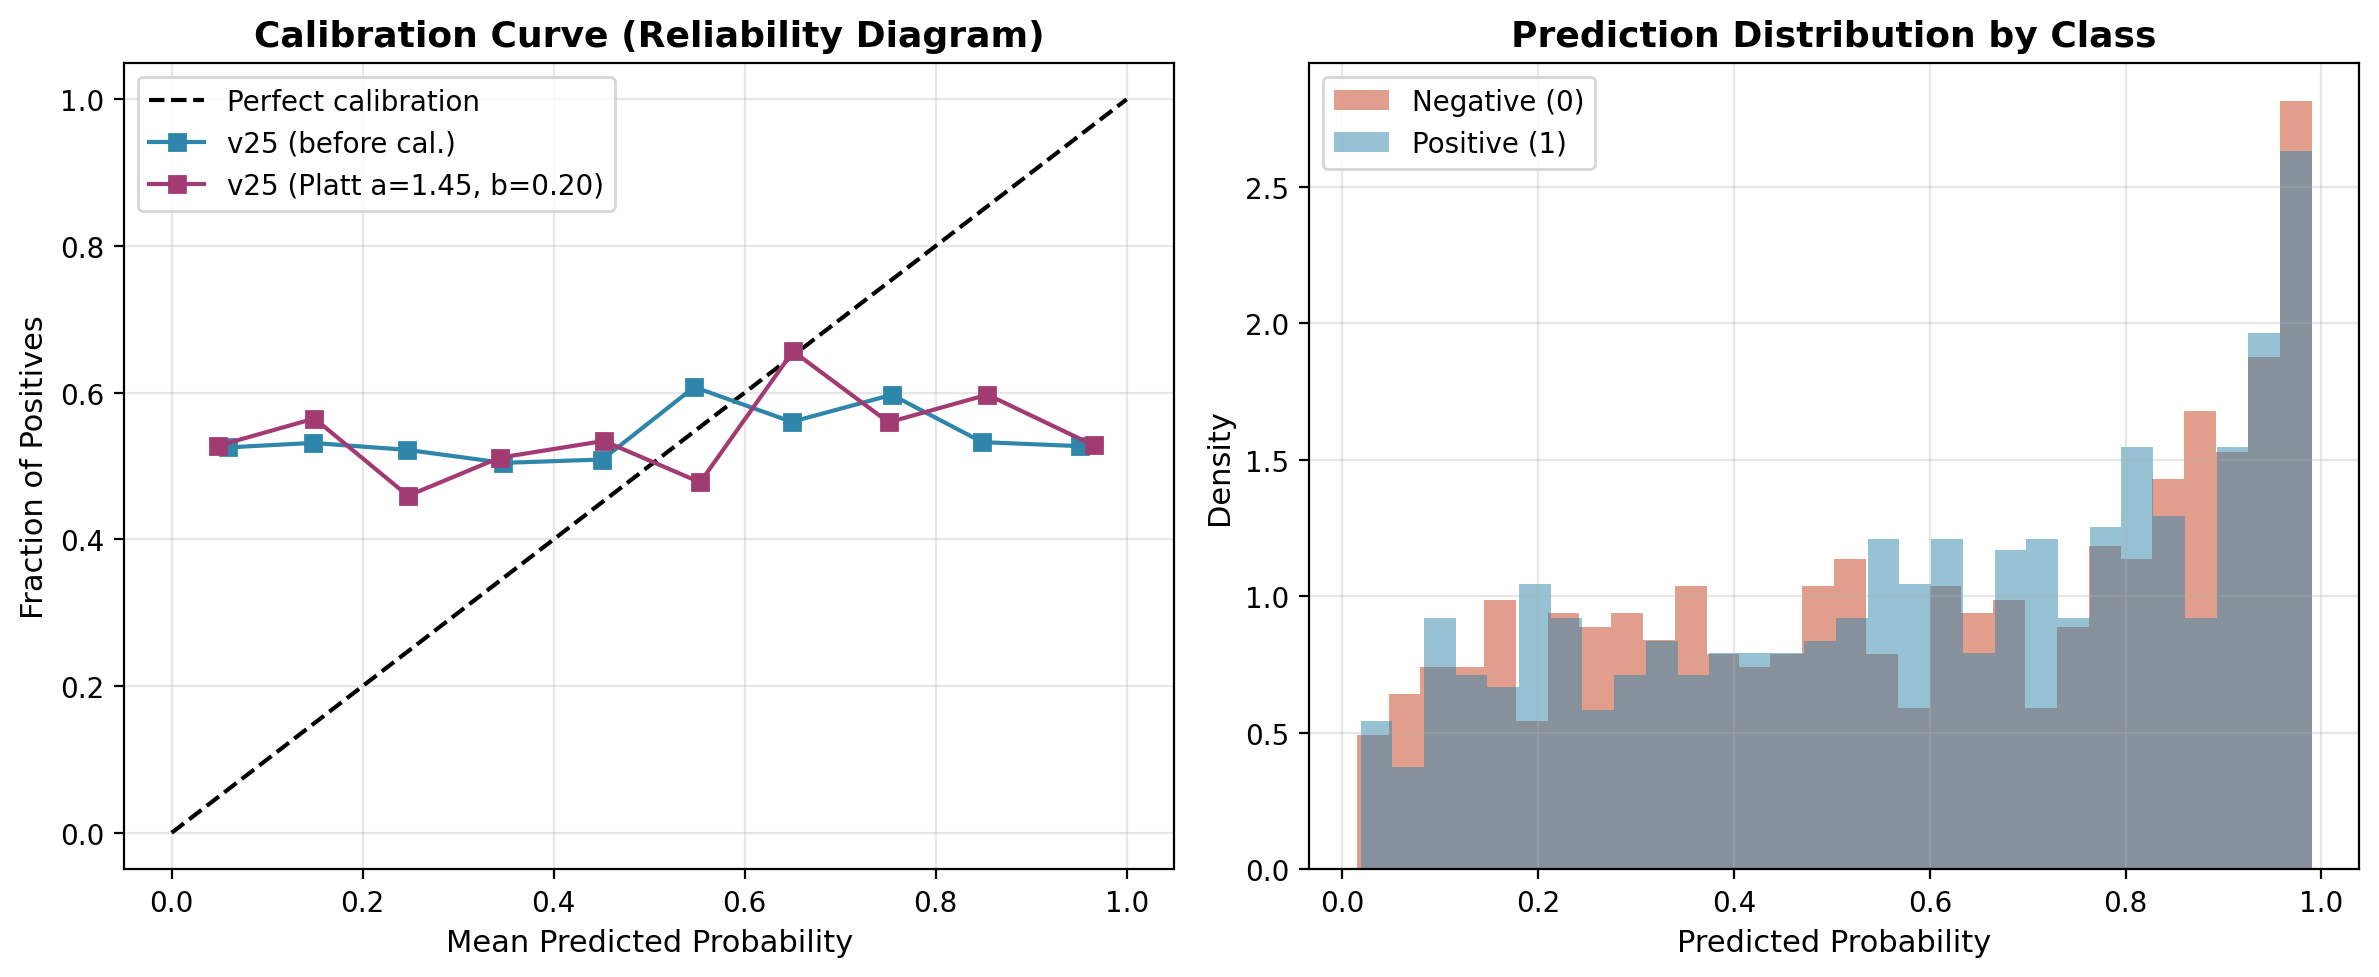
\includegraphics[width=0.9\linewidth]{figures/calibration.png}
    \caption{Calibration analysis. (Left) Reliability diagram: uncalibrated predictions (blue) show overconfidence; Platt-calibrated (red) align with perfect calibration line. (Right) Prediction density by class: good separation between negative (red) and positive (blue) classes.}
    \label{fig:calibration}
\end{figure}